%%
%% This is file `sample-sigconf.tex',
%% generated with the docstrip utility.
%%
%% The original source files were:
%%
%% samples.dtx  (with options: `sigconf')
%%
%% IMPORTANT NOTICE:
%%
%% For the copyright see the source file.
%%
%% Any modified versions of this file must be renamed
%% with new filenames distinct from sample-sigconf.tex.
%%
%% For distribution of the original source see the terms
%% for copying and modification in the file samples.dtx.
%%
%% This generated file may be distributed as long as the
%% original source files, as listed above, are part of the
%% same distribution. (The sources need not necessarily be
%% in the same archive or directory.)
%%
%% The first command in your LaTeX source must be the \documentclass command.
\documentclass[sigplan,10pt,anonymous,review]{acmart}


\providecommand{\tightlist}{%
  \setlength{\itemsep}{0pt}\setlength{\parskip}{0pt}}

%%
%% \BibTeX command to typeset BibTeX logo in the docs
\AtBeginDocument{%
  \providecommand\BibTeX{{%
    \normalfont B\kern-0.5em{\scshape i\kern-0.25em b}\kern-0.8em\TeX}}}

%% Rights management information.  This information is sent to you
%% when you complete the rights form.  These commands have SAMPLE
%% values in them; it is your responsibility as an author to replace
%% the commands and values with those provided to you when you
%% complete the rights form.

%%
%% Submission ID.
%% Use this when submitting an article to a sponsored event. You'll
%% receive a unique submission ID from the organizers
%% of the event, and this ID should be used as the parameter to this command.
%%\acmSubmissionID{123-A56-BU3}

%%
%% The majority of ACM publications use numbered citations and
%% references.  The command \citestyle{authoryear} switches to the
%% "author year" style.
%%
%% If you are preparing content for an event
%% sponsored by ACM SIGGRAPH, you must use the "author year" style of
%% citations and references.
%% Uncommenting
%% the next command will enable that style.
%%\citestyle{acmauthoryear}

%%
%% end of the preamble, start of the body of the document source.
\begin{document}

%%
%% The "title" command has an optional parameter,
%% allowing the author to define a "short title" to be used in page headers.
\title{Customizing Software by Direct Manipulation of Structured Data}

%%
%% The "author" command and its associated commands are used to define
%% the authors and their affiliations.
%% Of note is the shared affiliation of the first two authors, and the
%% "authornote" and "authornotemark" commands
%% used to denote shared contribution to the research.

\author{Geoffrey Litt}
\affiliation{%
  \institution{Massachusetts Institute of Technology}
  \city{Cambridge, MA}
  \country{USA}
}
\email{glitt@mit.edu}

\author{Daniel Jackson}
\affiliation{%
  \institution{Massachusetts Institute of Technology}
  \city{Cambridge, MA}
  \country{USA}
}
\email{dnj@csail.mit.edu}

%%
%% By default, the full list of authors will be used in the page
%% headers. Often, this list is too long, and will overlap
%% other information printed in the page headers. This command allows
%% the author to define a more concise list
%% of authors' names for this purpose.
% \renewcommand{\shortauthors}{Trovato and Tobin, et al.}

%%
%% The abstract is a short summary of the work to be presented in the
%% article.
\begin{abstract}
  In this paper we propose \emph{table-driven customization,} a new
  paradigm for enabling end users to customize software applications
  without doing traditional programming\emph{.} Users directly
  manipulate a tabular view of the structured data inside the
  application, rather than writing imperative scripts as in most
  customization tools. We extend this simple model with a spreadsheet
  formula language and custom data editing widgets, which provide
  sufficient expressivity to implement many useful customizations.

  We describe Wildcard, a browser extension which implements
  table-driven customization in the context of web applications. Through
  concrete examples, we demonstrate that this paradigm can be used to
  create useful customizations for real applications. We share
  reflections from our usage of the Wildcard system, including its
  strengths and limitations relative to other customization approaches.
  We further explore how new software architectures might encourage
  application developers to promote this style of end-user
  customization.
\end{abstract}

%%
%% The code below is generated by the tool at http://dl.acm.org/ccs.cfm.
%% Please copy and paste the code instead of the example below.
%%
%% From HERE
\begin{CCSXML}
<ccs2012>
<concept>
<concept_id>10011007.10011006.10011066.10011069</concept_id>
<concept_desc>Software and its engineering~Integrated and visual development environments</concept_desc>
<concept_significance>500</concept_significance>
</concept>
</ccs2012>
\end{CCSXML}

\ccsdesc[500]{Software and its engineering~Integrated and visual development environments}
% To HERE

%%
%% Keywords. The author(s) should pick words that accurately describe
%% the work being presented. Separate the keywords with commas.
\keywords{end-user programming, software customization, web browser extensions}

%% A "teaser" image appears between the author and affiliation
%% information and the body of the document, and typically spans the
%% page.
%\begin{teaserfigure}
%  \includegraphics[width=\textwidth]{sampleteaser}
%  \caption{Seattle Mariners at Spring Training, 2010.}
%  \Description{Enjoying the baseball game from the third-base
%  seats. Ichiro Suzuki preparing to bat.}
%  \label{fig:teaser}
%\end{teaserfigure}

%%
%% This command processes the author and affiliation and title
%% information and builds the first part of the formatted document.
\maketitle

\hypertarget{introduction}{%
\section{Introduction}\label{introduction}}

There have been many attempts at empowering end users to customize their
software by offering them a simplified programming tool. Some scripting
languages (AppleScript, Chickenfoot) have a friendly syntax that
resembles natural language. Visual programming tools (Mac Automator,
Zapier) eliminate text syntax entirely. Macro recorders (Applescript,
Helena, WebVCR) remove some of the initial programming burden by letting
a user start by concrete demonstrations.

These approaches have many differences, but they all share something in
common: an imperative programming model, with mutable variables,
conditionals and loops. End users ultimately must use these traditional
programming constructs to express their ideas, and the object of
interest is a \emph{script}, a sequence of commands.

We have known for decades about an alternate approach: \emph{direct
manipulation} \citep{shneiderman1983}, where ``visibility of the object
of interest'' replaces ``complex command language syntax''. Direct
manipulation is the de facto standard in GUIs today, but when it comes
to customizing software, it is rarely to be found. In this work, we ask:
what would it look like to build a software customization interface that
relies on direct manipulation? We take inspiration from spreadsheets and
visual database query interfaces \citep{2020a, bakke2016}, which have
successfully enabled end users to run queries and computations through
direct manipulation of data.

In this paper we present a technique called \emph{table-driven
customization} which applies these ideas from visual query interfaces in
the context of software customization. We augment an application's UI
with a table view, where the user can see and manipulate the structured
data inside an application. Changes in the table view result in
immediate corresponding changes to the original user interface of the
application, enabling the user to customize an application with live
feedback.

We have developed a browser extension called Wildcard which uses web
scraping techniques to implement table-driven customization for existing
Web applications. In Section~\ref{sec:examples} we concretely introduce
the key ideas of table-driven customization by presenting several
examples of real customizations implemented in Wildcard.

In Section~\ref{sec:architecture} we explain the architecture of
table-driven customization. We focus on the \emph{table adapter}
abstraction, which allows many different types of underlying state to be
bidirectionally mapped to a table of data. We describe certain types of
table adapters we've built in Wildcard; we also describe future adapters
that could be supported in the general paradigm.

We have used Wildcard to build real customizations for 11 different
websites. In Section~\ref{sec:evaluation} we present reflections from
this process: customizations we were able to build, limitations we
encountered, and reflections on the ease of integrating scraping logic
with real websites.

In Section~\ref{sec:themes}, we discuss some key themes from our work:

\begin{itemize}
\tightlist
\item
  \emph{Customization by direct manipulation}: End users should be able
  to customize an application by examining and modifying its data,
  rather than by writing imperative scripts.
\item
  \emph{Third-party semantic wrappers}: Typically, tools that don't rely
  on official extension APIs resort to offering low-level APIs for
  customization. Instead, we suggest a community-maintained library of
  semantic wrappers around existing applications, enabling end users to
  work with domain objects rather than low-level representations.
\end{itemize}

Table-driven customization relates to existing work in many areas. In
particular, our goals overlap with many software customization tools,
and our methods overlap with direct manipulation interfaces for working
with structured data, including visual database query systems and
spreadsheets. We explore these connections and more in
Section~\ref{sec:related-work}.

\hypertarget{sec:examples}{%
\section{Examples}\label{sec:examples}}

\emph{todo: maybe redo this as a separate example to avoid self
plagiarism?}

To concretely illustrate the end user experience of table-driven
customization, here are several real examples of using the Wildcard
browser extension to customize websites.

\begin{figure*}
\hypertarget{fig:airbnb-demo}{%
\centering
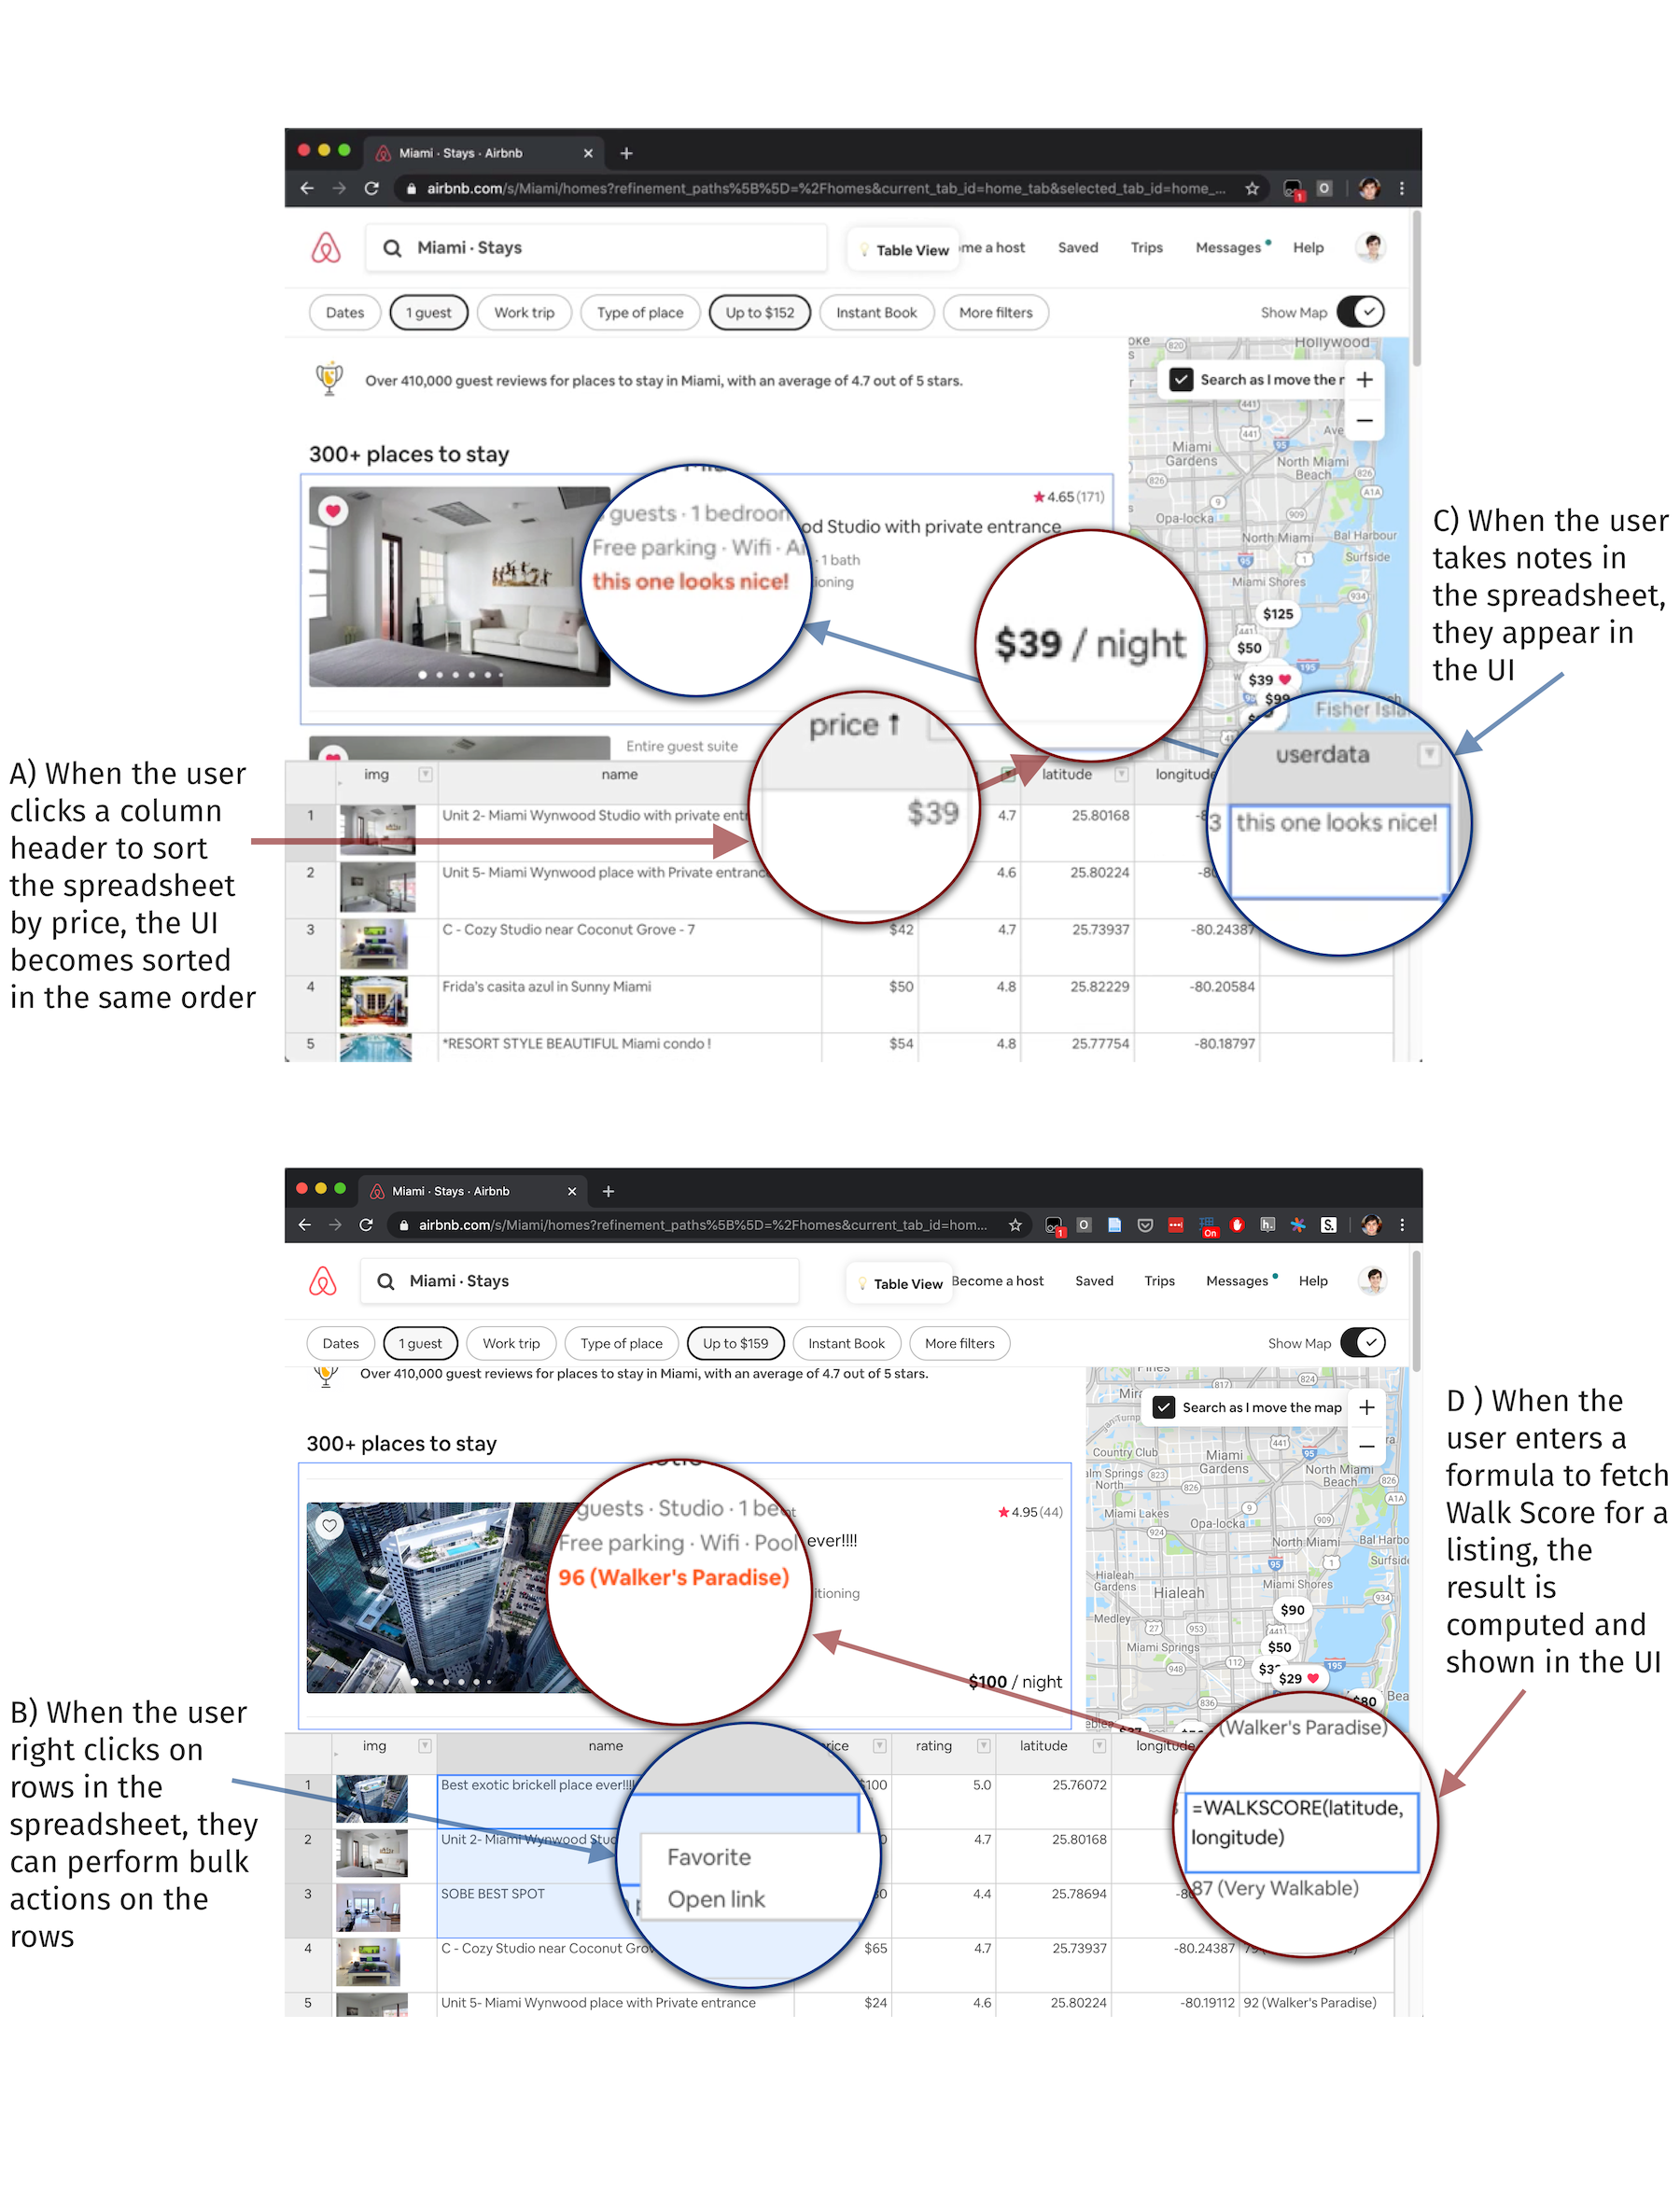
\includegraphics{media/airbnb-demo-300dpi.png}
\caption{Using Wildcard to augment the Airbnb search page for booking
accommodations}\label{fig:airbnb-demo}
}
\end{figure*}

\hypertarget{augmenting-search-results}{%
\subsection{Augmenting search results}\label{augmenting-search-results}}

In 2012, the travel site Airbnb removed the ability to sort
accommodation searches by price. Users could still filter by price
range, but could no longer view the cheapest listings first. Many users
complained that the change seemed hostile to users. ``It's so
frustrating! What is the logic behind not having this function?'' said
one user on the
\href{https://community.withairbnb.com/t5/Hosting/Sorting-listing-by-price/td-p/559404}{Airbnb
support forum}. Alas, the feature remains missing to this day.

Using Wildcard, the user can fix this omission, while leaving the page's
design and the rest of its functionality unchanged.{
Figure~\ref{fig:airbnb-demo} shows an overview of augmenting the Airbnb
site.} First, the user opens up the Wildcard panel, which shows a table
corresponding to the search results in the page. As they click around in
the table, the corresponding row in the page is highlighted to indicate
the mapping between the views.

Then, the user clicks on the price column header to sort the spreadsheet
and the Airbnb UI by price{ (Figure~\ref{fig:airbnb-demo}, Note A)}.
They also filter to listings with a user rating above 4.5 (another
feature missing in the original Airbnb UI).

After manipulating the data, the user closes the table view and
continues using the website. Because the application's UI usually has a
nicer visual design than a spreadsheet, Wildcard does not aim to replace
it---at any time, the user can use either the UI, the spreadsheet, or
both together.

Many websites that show lists of data also offer actions on rows in the
table, like adding an item to a shopping cart. Wildcard has the ability
to make these ``row actions'' available in the data table through the
site adapter. In the Airbnb UI, saving multiple listings to a Favorites
list requires tediously clicking through them one by one. Using Wildcard
row actions, the user can select multiple rows and favorite all of them
with a single click{ (Figure~\ref{fig:airbnb-demo}, Note B)}. Similarly,
the user can open the detailed pages for many listings at once.

Next, the user wants to jot down some notes about each listing. To do
this, they type some notes into an additional column in each row, and
the notes appear inside the listings in the original UI{
(Figure~\ref{fig:airbnb-demo}, Note C)}. The annotations are saved in
the browser and associated with the backend ID of the listing, so they
will appear in future browser sessions that display the same listing.

Wildcard also includes a formula language that enables more
sophisticated customizations. When traveling without a car, it's useful
to evaluate potential places to stay based on how walkable the
surroundings are. Using a formula, the user can integrate Airbnb with
Walkscore, an API that rates the walkability of any location on a 1-100
scale. When the user calls the \texttt{walkscore} formula with the
listing's latitude and longitude as arguments, it returns the walk score
for that location and shows it as the cell value. Because the cell's
contents are injected into the page, the score also appears in the UI{
(Figure~\ref{fig:airbnb-demo}, Note D)}.

\hypertarget{snoozing-todos}{%
\subsection{Snoozing todos}\label{snoozing-todos}}

\begin{figure*}
\hypertarget{fig:airbnb-demo}{%
\centering
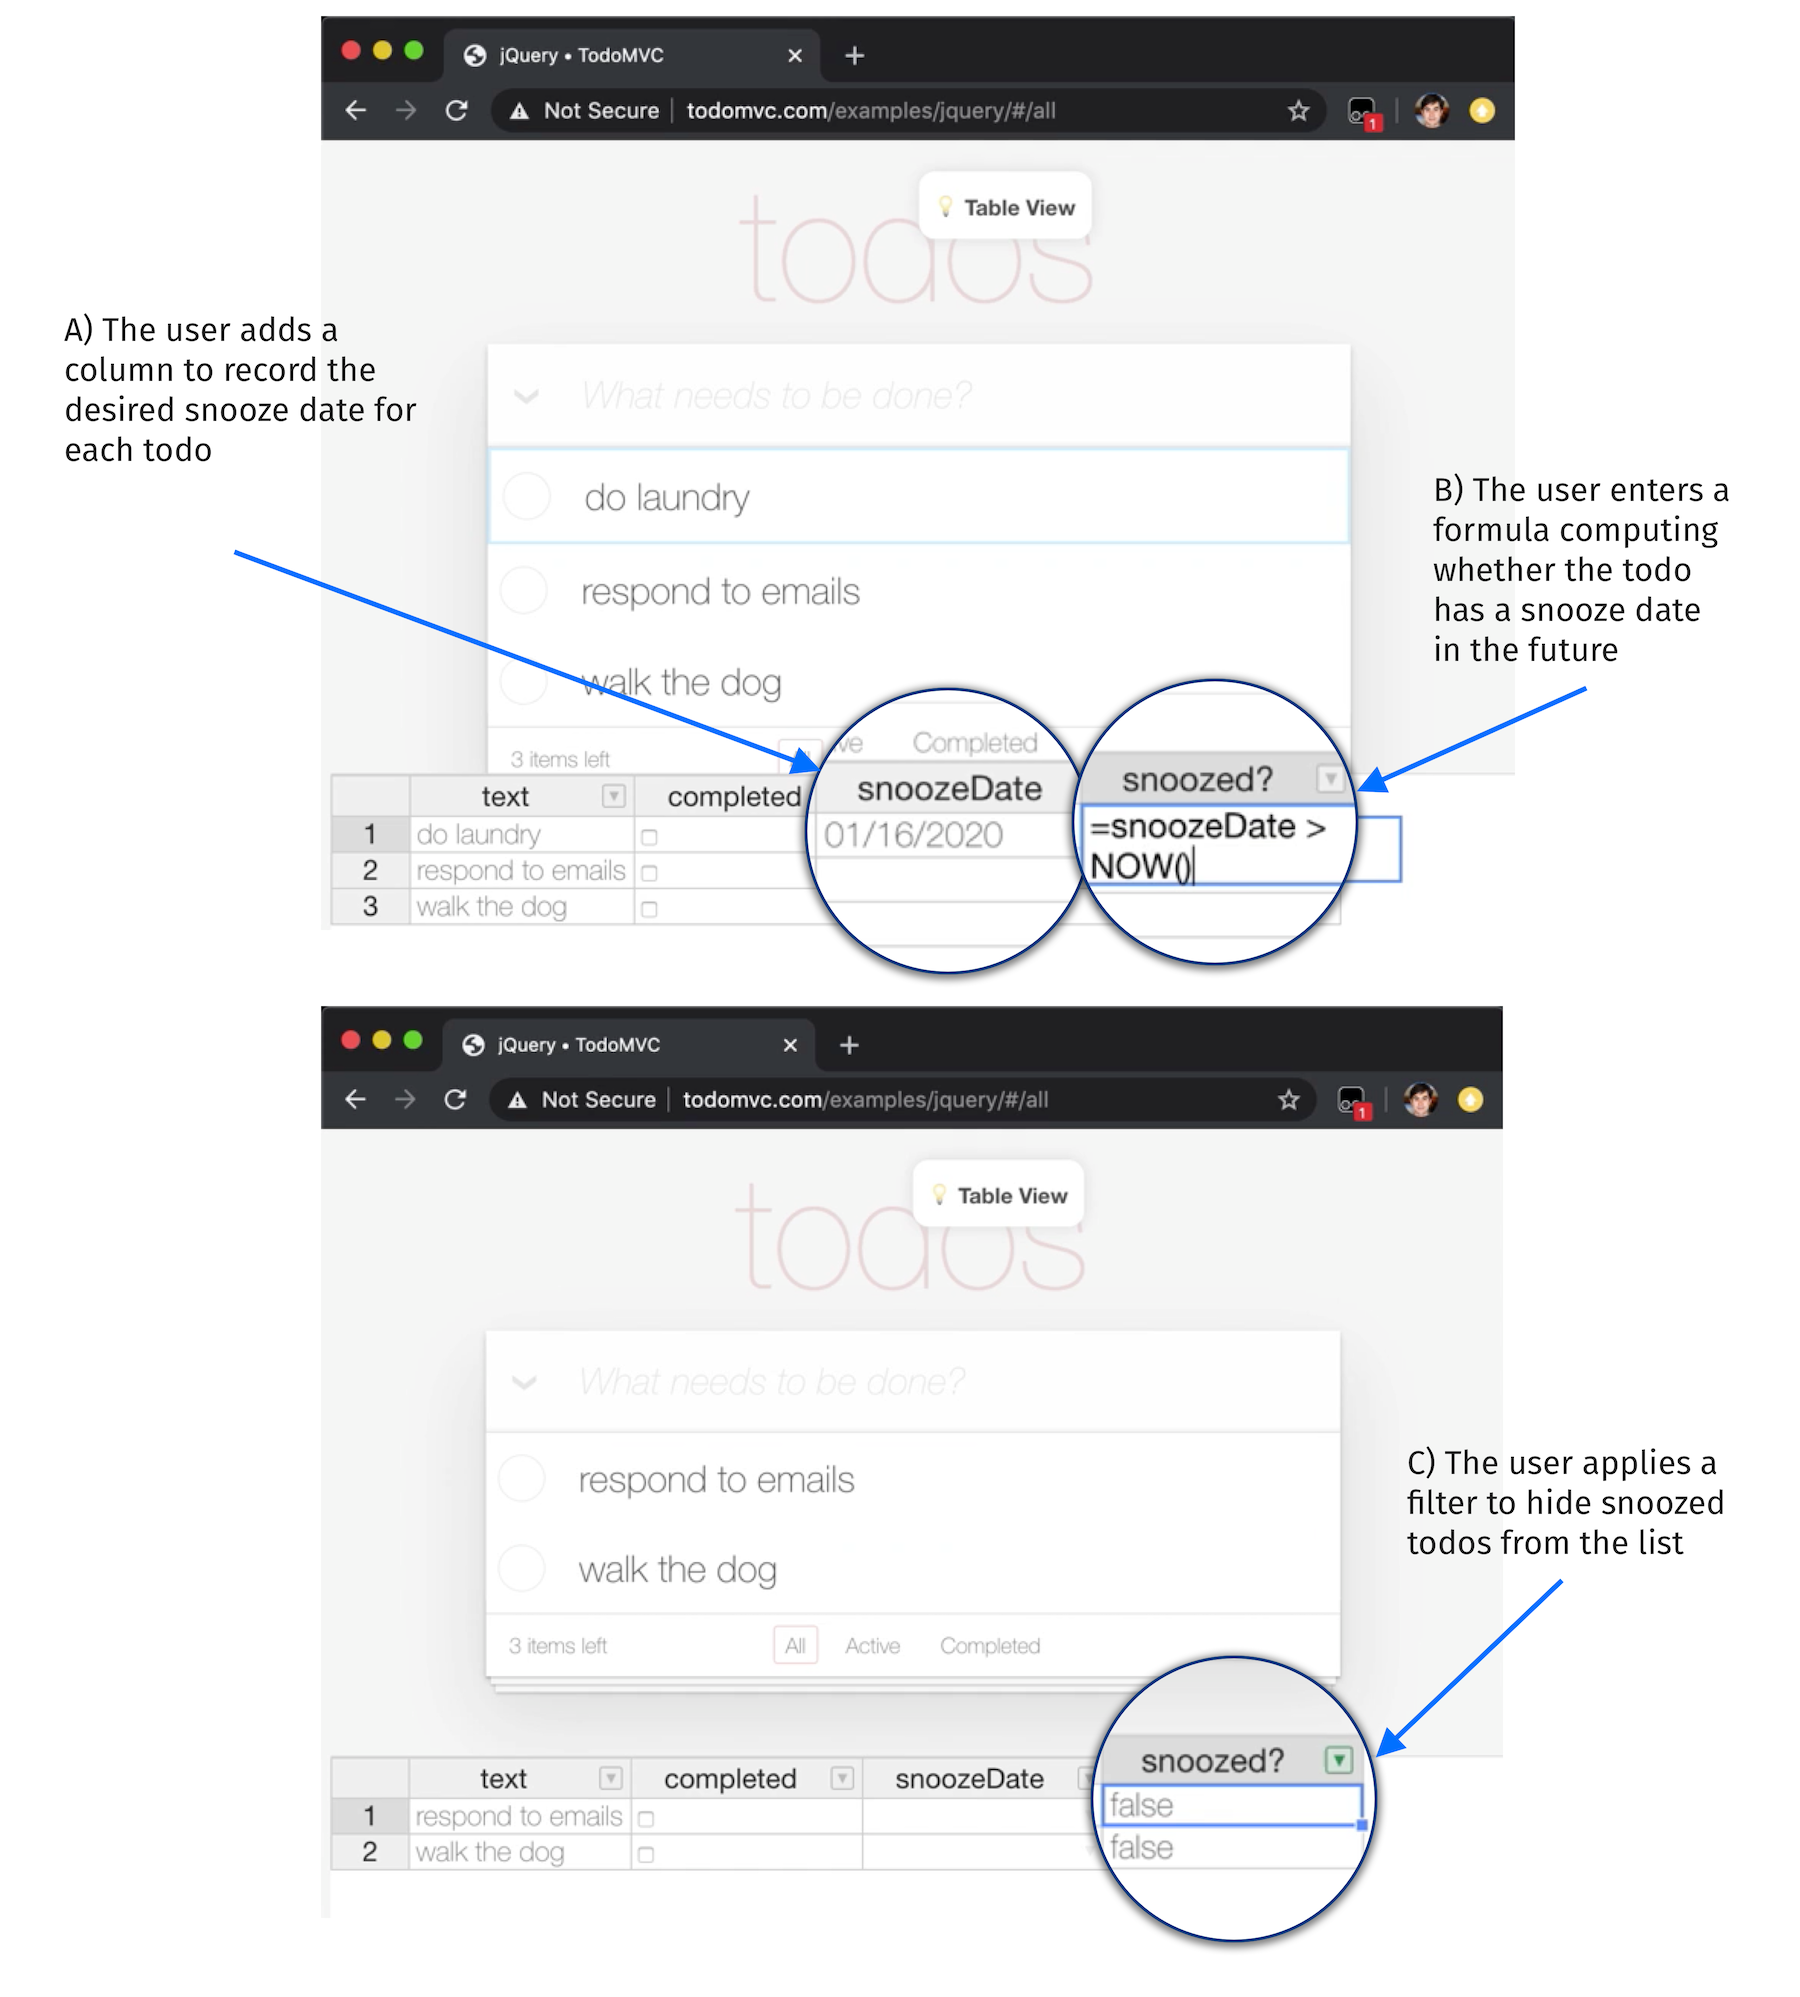
\includegraphics{media/todomvc-demo-300dpi.png}
\caption{Using Wildcard to add a "snooze" feature to the TodoMVC todo list app}\label{fig:todomvc-demo}
}
\end{figure*}

In addition to fetching data from other sources, Wildcard formulas can
also perform computations. In this example, the user would like to
augment the TodoMVC todo list app with a ``snooze'' feature, which will
temporarily hide a todo from the list until a certain date.{
Figure~\ref{fig:todomvc-demo} shows an overview of this customization.}

The user opens the table view, which shows the text and completed status
of each todo. They start the customization by adding a new column to
store the snooze date for each todo{ (Figure~\ref{fig:todomvc-demo},
Note A)}.

The next step is to hide snoozed todos. The user creates a
\texttt{snoozed?} column, which uses a formula to compute whether a todo
is snoozed---i.e., whether it has a snooze date in the future{
(Figure~\ref{fig:todomvc-demo}, Note B)}. Then, they simply filter the
table to hide the snoozed todos{ (Figure~\ref{fig:todomvc-demo}, Note
C)}.

Because the built-in \texttt{NOW()} function always returns the current
datetime, snoozed todos will automatically appear once their snooze date
arrives.

Because this implementation of snoozing was built on the spreadsheet
abstraction, it is completely decoupled from this particular todo list
app. We envision that users could share these types of customizations as
generic browser extensions, which could be applied to any site supported
by Wildcard with no additional effort.

\hypertarget{adding-a-custom-datepicker}{%
\subsection{Adding a custom
datepicker}\label{adding-a-custom-datepicker}}

\begin{figure*}
\hypertarget{fig:airbnb-demo}{%
\centering
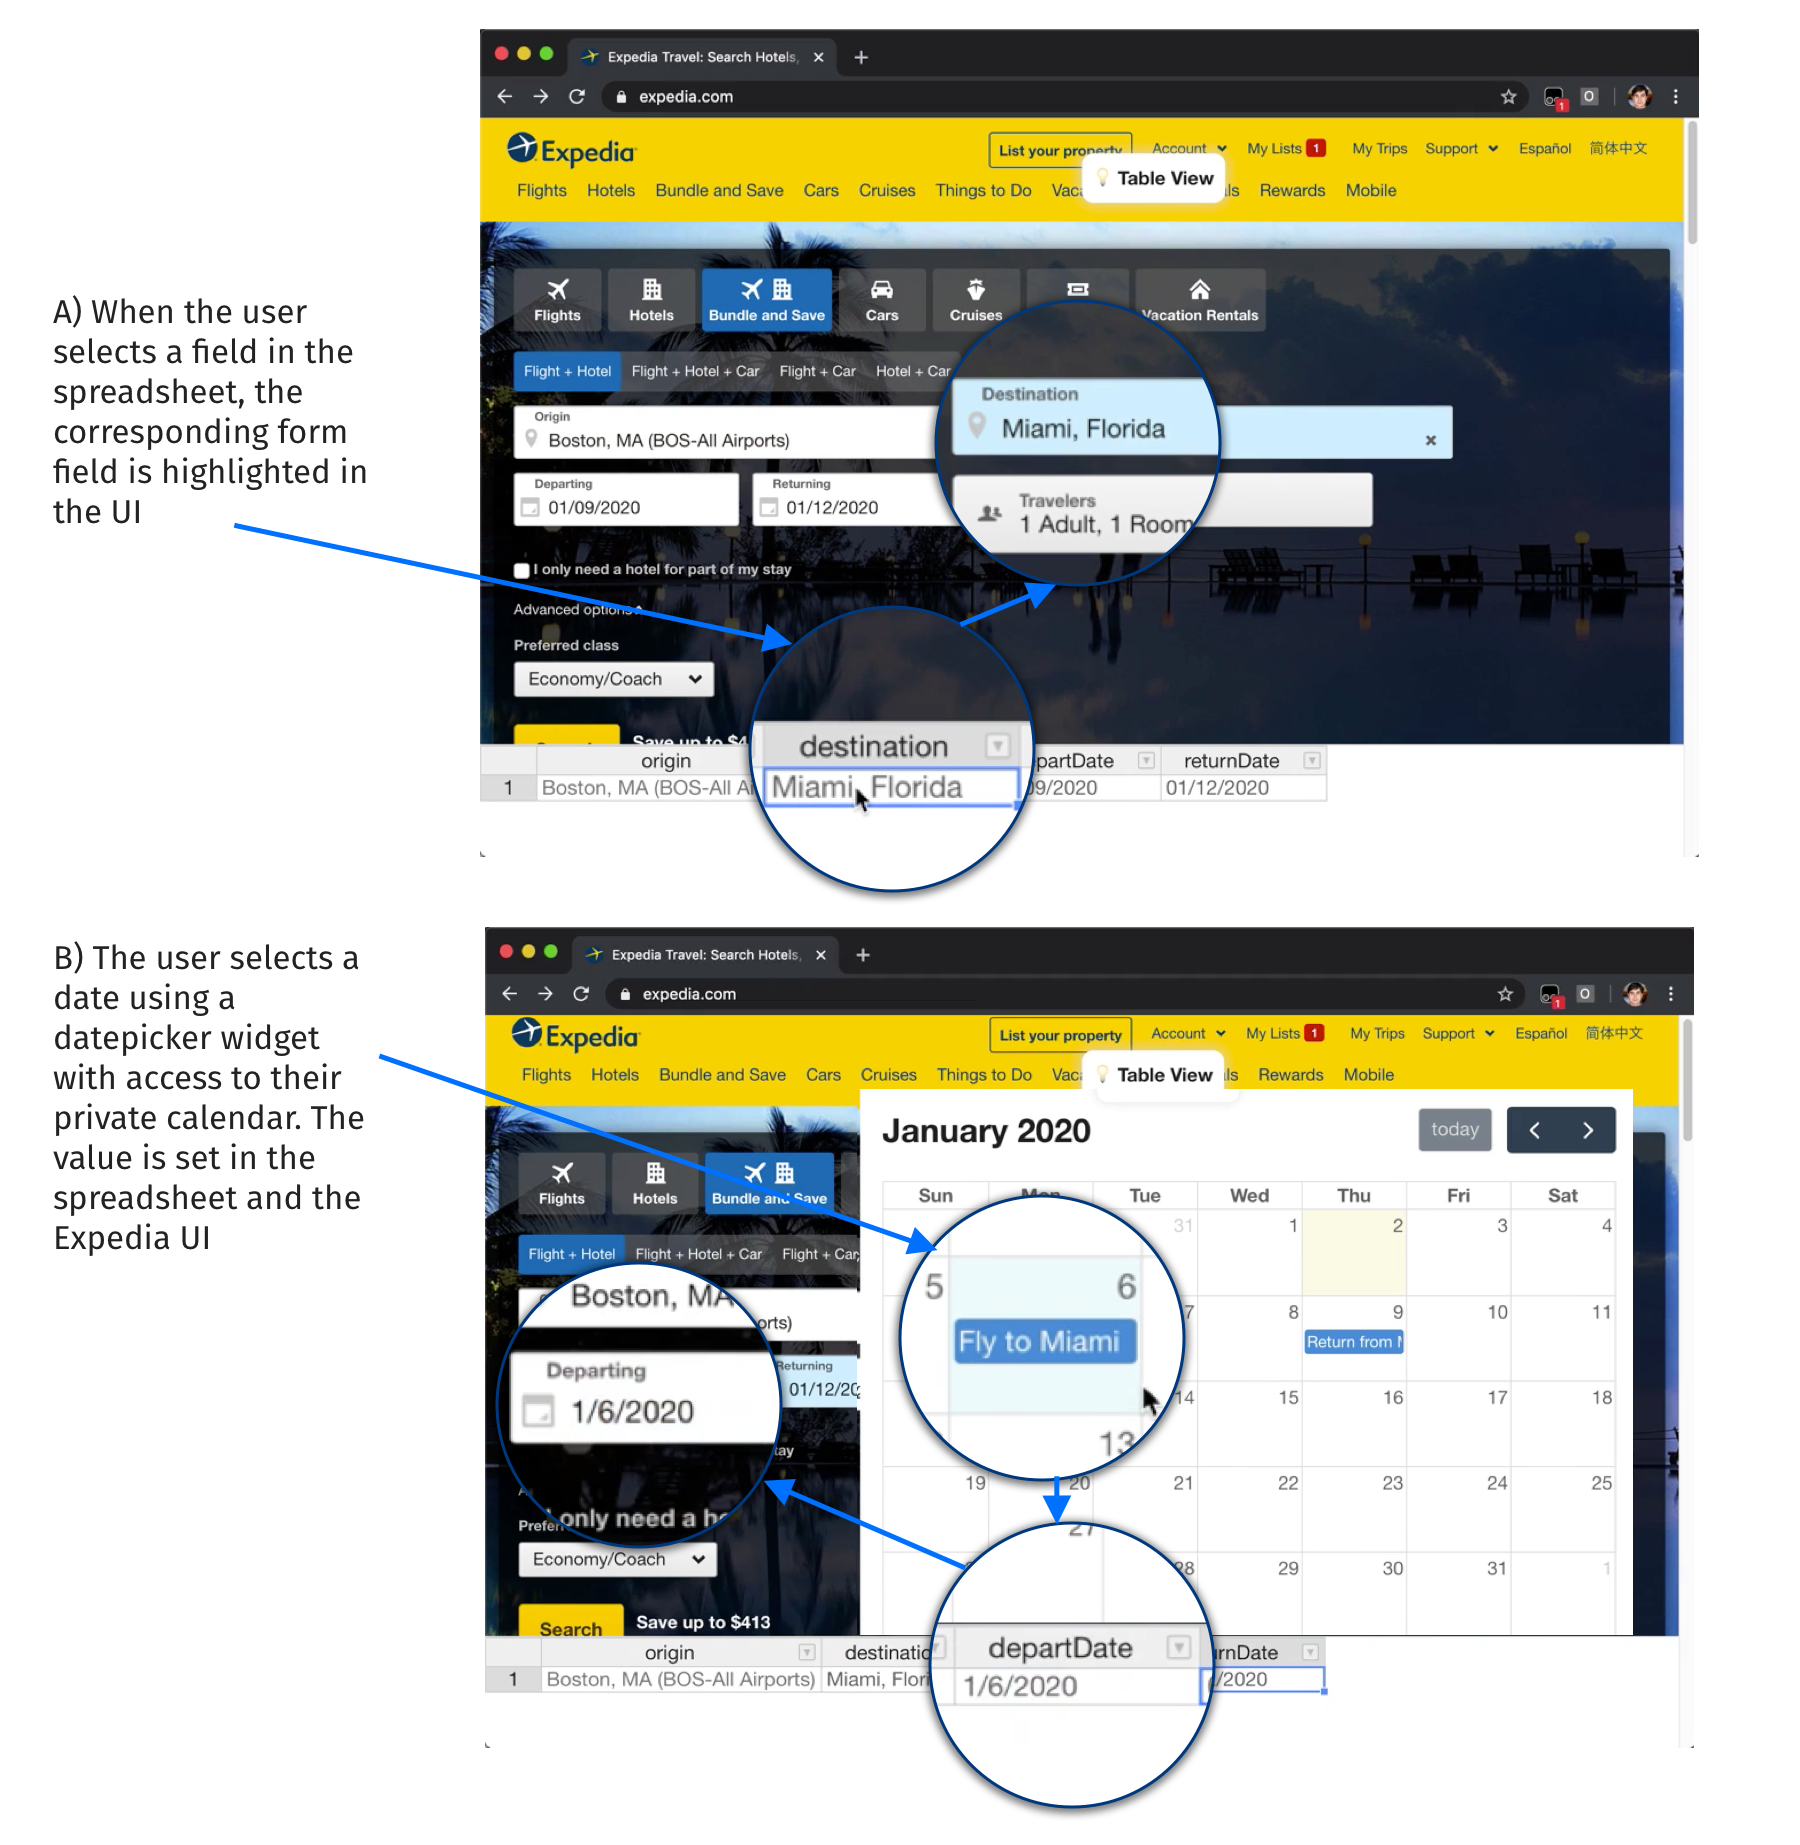
\includegraphics{media/expedia-demo-300dpi.png}
\caption{Using Wildcard to augment the Expedia page for booking a flight}\label{fig:expedia-demo}
}
\end{figure*}

It might seem that Wildcard is only useful on websites that display
lists of tabular data, but the table metaphor is flexible enough to
represent many types of data. For example, a flight search form on
Expedia can be represented as a single row, with a column corresponding
to each input{ (Figure~\ref{fig:expedia-demo}, Note A)}.

In some of the previous examples, the table cells were read-only
(because users can't, for example, change the name or price of an Airbnb
listing). In this case, the cells are writable, which means that changes
in the table are reflected in the form inputs. This becomes especially
useful when combined with GUI widgets that can edit the value of a table
cell.

Filling in dates for a flight search often requires a cumbersome
workflow: open up a separate calendar app, find the dates for the trip,
and then carefully copy them into the form. In Wildcard, the user can
avoid this by using a datepicker widget that shows the user's personal
calendar events{ (Figure~\ref{fig:expedia-demo}, Note B)}. The user can
directly click on the correct date, and it gets inserted into both the
spreadsheet and the original form.n

\hypertarget{sec:architecture}{%
\section{System architecture}\label{sec:architecture}}

\begin{figure}
\hypertarget{fig:table-adapter}{%
\centering
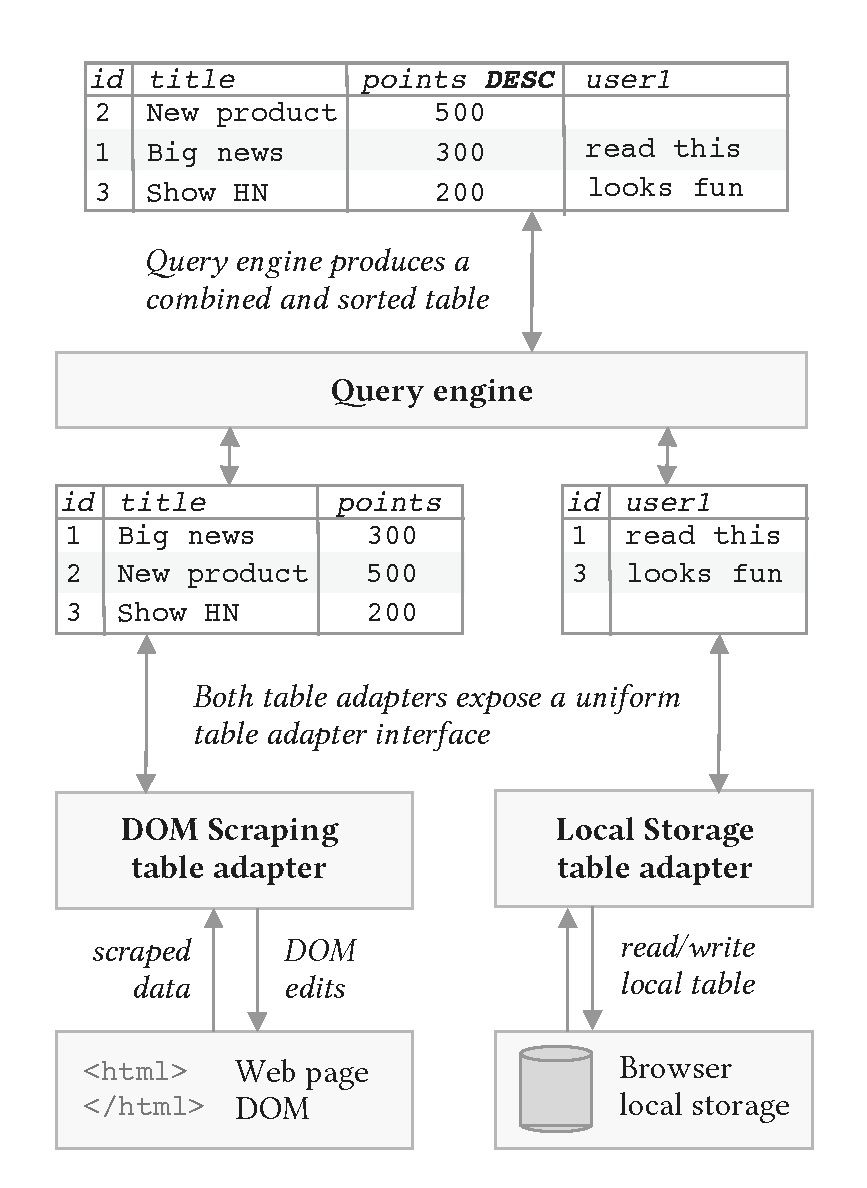
\includegraphics[width=\columnwidth]{media/table-adapter.eps}
\caption{The table adapter architecture}\label{fig:table-adapter}
}
\end{figure}

Figure~\ref{fig:table-adapter} summarizes the overall architecture of
table-driven customization, using a simplified version of the Airbnb
example above. In this example, the name of each listing is scraped from
the web page DOM, the latitude and longitude of each listing is scraped
from AJAX responses, and user annotations are loaded from the brower's
local storage.

First, the three different data sources are each bidirectionally mapped
to a table interface by a \textbf{table adapter}. The table adapter
defines how to map a particular type of data to a table, and what
effects edits should have on the original data source. In some cases,
the mapping logic is straightforward: the local storage adapter stores a
table of data, so the mapping to the table abstraction is trivial. In
other cases, the mapping is more involved: the DOM scraping adapter
implements web scraping logic to produce a table of data from the web
page, and edits to the table result in DOM manipulations like reordering
rows of data on the page.

Ultimately, we provide the user with a single combined table view that
they can edit, rather than three separate tables. The \textbf{query
engine} is responsible for combining the tables of data into this single
view, and routing the user's edits back to the individual table
adapters. In this example, the query engine has joined the three tables
together by a shared ID column, and sorted the result by the name
column.

We now examine each component of the system in more detail.

\hypertarget{table-adapters}{%
\subsection{Table adapters}\label{table-adapters}}

A key idea in table-driven customization is that different data sources
can all be mapped to the generic abstraction of an editable table. In a
relational database, the table matches the underlying storage format,
but in table-driven customization, the table is merely an
\emph{interface layer}. The data shown in the table is a projection of
some underlying state, and edits to the table can have arbitrary effects
on the underlying state.

Externally, a table adapter must satisfy an abstract interface. The
first two parts of the interface largely resemble the interface exposed
by a table in a relational database:

\textbf{Returning a table}: A table adapter exposes a table of data: an
ordered list of records. Each record contains associates attributes and
values. Tables have a typed schema, so the same attributes are shared
across all records. A table adapter can update the contents of a table
at any time, in response to changes in the underlying state (e.g., a DOM
scraping adapter can update the table when the page body changes). New
data is pushed out to other components of the system, and the query view
reactively updates in response.

\textbf{Making edits}: The query engine can request to a table adapter
to make an edit to a record. The meaning of making an edit can vary
depending on the adapter: in the local storage adapter, an annotation
can be persisted into local storage; in the DOM scraping adapter, an
edit can represent filling in a form field. An adapter can also mark
values as read-only if it wouldn't be meaningful to edit them; for
example, the DOM scraping adapter typically marks page content as
read-only, except for editable form fields.

The query engine also sends additional information about the combined
query view to each table adapter. These functions are currently used to
provide the DOM scraping adapter with sufficient information to
manipulate the original application UI as the user manipulates the table
view.

\textbf{Sorting/filtering}: When the user sorts or filters the query
view, an ordered list of visible IDs is sent to each table adapter. The
DOM scraping adapter uses this information to modify the list of visible
rows in the web page.

\textbf{Information from other tables}: The query engine sends each
table adapter the entire combined table of data being rendered to the
user. The DOM scraping adapter uses this to add annotations to the page
by looking for additional data columns joined to scraped rows, and
rendering them in the page.

\textbf{Currently selected record}: The query engine notifies each table
adapter about which record is currently selected by the user in the
table UI. The DOM scraping adapter uses this information to highlight
the row in the page that corresponds to the selected record in the
table.

\hypertarget{types-of-table-adapters}{%
\subsubsection{Types of table adapters}\label{types-of-table-adapters}}

Here we describe in more detail the table adapters which we have
implemented in Wildcard to power the customizations shown in
Section~\ref{sec:examples}.

\textbf{DOM scraping adapters} are the essential component that enables
Wildcard to interface with an existing website UI. In addition to the
standard web scraping problem of extracting a table of data from the
DOM, a scraping adapter must also manipulate the DOM to re-order rows,
edit form entries, and inject annotations as the table is edited.

Because each website has unique content, we rely on programmers to
create a DOM scraping adapter for each individual website to make it
available for customization in Wildcard. To make this approach viable,
we have built library functions that make it as easy as possible to
implement a scraping adapter, only requiring the programmer to implement
the minimal site-specific parts. The programmer writes a single scraping
function which uses CSS selectors and DOM APIs to extract and return
relevant elements from the page. The library functions then wrap this
function to implement the rest of the needed functionality; for example,
when the table is sorted, we find the DOM elements corresponding to the
rows in the table, remove them from the page, and then reinsert them in
the new order.

An \textbf{AJAX scraping adapter} intercepts AJAX requests made by a web
page, and extracts information from those requests. When available, this
tends to be a helpful technique because the data is already in a
structured form, and often includes information not shown in the UI. As
with DOM scraping adapters, we have made it as easy as possible for
programmers to create site-specific AJAX scraping adapters. A programmer
writes a function which specifies how to extract data from an AJAX
request, and the framework handles the details of actually intercepting
requests and calling the programmer-defined function.\footnote{So far we
  have only implemented AJAX scraping in the Firefox version of
  Wildcard, since Firefox has convenient APIs for intercepting requests.
  It appears possible to implement in Chrome as well, but we have not
  finished our implementation.}

The \textbf{local storage adapter} simply stores a table of data in the
browser. As shown in the example use cases, this can be useful for
privately persisting annotations, without needing to upload them to a
web service.

\hypertarget{future-adapters}{%
\subsubsection{Future Adapters}\label{future-adapters}}

We have designed the table adapter API to be general enough to support
other types of useful adapters in the future. Here are three examples of
future possibilities:

\textbf{Integrated website adapters}: A key benefit of the table adapter
abstraction is that Wildcard is not coupled to web scraping as the only
means for integrating with existing sites, but can also accommodate
first party developers adding support directly into their own websites.
A DOM Scraping table adapter could be swapped out for an ``integrated
website adapter'' which directly accesses the internal state of the
application, without needing to extract it from the UI.

With the advent of rich frontend web frameworks, structured application
state is now often available in the web client. We suspect it is
possible to create plugins for frontend frameworks which expose
structured state to Wildcard with minimal effort from the application
developers. For example, we have created an initial prototype of a
plugin for the Redux state management library, which represents the
state of a user interface as a single object. To configure an integrated
website adapter for such an existing application, the user simply
specifies two functions. The first one projects the centralized
application state into a table, and define handlers for how data edits
to the table should affect the state.

\textbf{Shared storage adapter}: It would be useful to share user
annotations between people and across devices---for example,
collaboratively taking notes with friends on a list of options for
places to stay on Airbnb. The existing Local Storage Adapter could be
extended to share live synchronized data with other users. This could be
achieved through a centralized web server, or through P2P connections
which might provide stronger privacy guarantees.

\textbf{Third party API data adapter}: Currently, the main mechanism for
including data from web APIs in Wildcard is using spreadsheet formulas.
However, a web API could also be wrapped to expose a table API that
would dynamically create tables in response to queries. For example,
when fetching walkability scores for many GPS locations, the query
engine could request a table of walkability scores for various pairs of
latitude and longitude, and the table adapter could dynamically perform
API queries to populate a result table. (\emph{todo: make a stronger
case for why this is useful or better than formulas})

(\emph{note: another ordering for the adapters could be by function.
First, DOM, AJAX, and Redux, which all integrate with the original app.
Then, Local Storage, Shared Storage, API, which are all about adding
functionality to the site. This might make more logical sense, but it
risks confusing what's already been done and what's a future
possibility. The current order seems good enough?})

\hypertarget{query-engine}{%
\subsection{Query engine}\label{query-engine}}

The query engine is responsible for coordinating across multiple table
adapters. It joins data across multiple tables and creates a single
result table which is shown to the user through the editor. It also
handles all user interactions and routes appropriate messages to each
table adapter.

First, every query involves a primary DOM scraping table adapter which
associates records in the result with elements in the application's user
interface. At minimum, the primary table adapter needs to return record
IDs and have the ability to manipulate the application's UI. It can also
optionally return data about each record.

Next, additional tables (AJAX data, local storage data) are left joined
by ID. (\emph{todo: discuss IDs here?}) Finally, the result table can be
sorted and filtered by any column.

One way to think of this model is a tiny constrained subset of the SQL
query model. We've found that this simple model has proven sufficient
for meeting the needs of customization in practice, and minimizes the
complexity of supporting more general and arbitrary queries. But because
it fits into the general SQL paradigm, it could theoretically be
extended to support more types of queries.

The query engine is also responsible for executing formulas. We have
built a small language resembling the formula languages in visual query
tools like SIEUFERD. As in those tools, and unlike in spreadsheets,
formulas automatically apply to an entire column of data, and can
reference columns rather than only specific cells.

\hypertarget{table-editor}{%
\subsection{Table editor}\label{table-editor}}

In Wildcard we provide a basic table editor as the user interface on top
of the query engine. It is built with the Handsontable Javascript
library, which provides UI elements for viewing and editing a table, as
well as basic query operations like sorting and filtering.

\emph{todo: other table instruments}

\hypertarget{sec:themes}{%
\section{Key themes}\label{sec:themes}}

\hypertarget{customization-by-direct-manipulation}{%
\subsection{Customization by direct
manipulation}\label{customization-by-direct-manipulation}}

Hutchins, Hollan and Norman \citep{hutchins1985} describe a direct
manipulation interface as one that uses a model-world metaphor, rather
than a conversation metaphor. Rather than conversing with the system
about an assumed world, ``the world is explicitly represented'' and the
user can ``{[}act{]} upon the objects of the task domain themselves.''

Most GUIs today employ direct manipulation, but software customization
tools typically use an imperative programming model, which implements
the conversational metaphor rather than direct manipulation. For
example, in Applescript \citep{cook2007}, the scripting language for
customizing Mac OS applications, here is how a user retrieves a list of
of calendar names from the Calendar application:

\begin{verbatim}
tell application "Calendar"
  name of calendars
end tell
\end{verbatim}

Some customization environments (Mac Automator, Zapier) forego text
syntax and enable the user to connect programs and construct automations
by dragging and dropping commands. These environments still do not
constitute direct manipulation, though: the objects being manipulated
are in the domain of programming, not the domain of the task at hand.

It is reasonable to choose imperative programming as the model for
building customizations. Turing-Complete programming provides a high
ceiling for possible customizations, and the a sequence of commands is a
natural fit for automations which simulate a series of steps taken by
the user.

However, there is a serious drawback to this approach. MacLean et al
\citep{maclean1990} describe an ideal for user-tailorable systems: a
``gentle slope'' from using to customizing, where small incremental
increases in skill lead to corresponding increments of customization
power. Requiring users to learn programming for customization creates an
abrupt ``cliff,'' where a significant learning investment is required
even to implement simple customizations. Another goal of MacLean et al
is that ``it should be as easy to change the environment as it is to use
it,'' at least for some subset of changes. In scripting languages, even
user-friendly ones like Applescript or Chickenfoot, the experience of
customization does not remotely resemble the experience of use, so these
systems can't meet this goal.

With table-driven customization we aim to provide a gentler slope, by
using direct manipulation for software customization. The data shown in
the table view is the domain data from the original application. The
user makes changes to the data by selecting areas of interest in the
table, e.g.~sorting/filtering by clicking the relevant column header, or
adding annotation by clicking on the relevant row. These interactions
are common in GUI applications, and Wildcard therefore meets MacLean et
al's goal: some one-click customizations are as easy as using the
original application.

One aspect of directness which we have chosen not to maintain in
Wildcard is enabling customization in the context of the original user
interface, as explored by some other tools like Scotty
\citep{eagan2011}. We have found that augmenting the original UI with an
additional structured representation has numerous benefits. It provides
a consistent experience across all applications, and clearly shows the
user what structured data is available to work with.

Ainsworth et al's provide a helpful taxonomy of the value of multiple
representations \citep{ainsworth1999}. In their terms, Wildcard plays a
\emph{complementary role} by supporting a different set of tasks from
the original application, while displaying \emph{shared information}. We
also suspect that Wildcard helps \emph{constructs deeper understanding}
by \emph{subtraction}. By stripping away details and only showing the
essential data in an interface, Wildcard helps users think of new ways
of using that data, outside the specific constraints of the original
application.

It is important to note that there are many specific customizations that
can be achieved in systems like Chickenfoot \citep{bolin2005} that
cannot be reproduced in Wildcard. We consider this an acceptable
tradeoff in exchange for achieving a gentler slope of customization, and
we show in Section~\ref{sec:examples} and Section~\ref{sec:evaluation}
that our model can still implement many useful customizations in
practice. Also, there is sometimes a way to reframe an imperative script
in terms of our direct manipulation model; for example, a script that
iterates through rows in a page adding some additional information could
be reproduced using a formula in Wildcard.

\hypertarget{third-party-semantic-wrappers}{%
\subsection{Third-party semantic
wrappers}\label{third-party-semantic-wrappers}}

Software customization tools typically fall into one of two categories:
third-party, or semantic.

\emph{Third-party customization tools} enable customization without
using official extension APIs, enabling a broader range of
customizations on top of more applications. For example, web browser
extensions have demonstrated the utility of customizing websites through
manipulating the DOM, without needing explicit extension APIs to be
built in. However, third-party customization comes with a corresponding
cost: these tools can typically only operate at a low level of
abstraction, e.g.~manipulating user interface elements. This makes it
harder for end users to write scripts, and makes the resulting scripts
more brittle. (todo: support this claim more, provide examples)

\emph{Semantic customization tools} use explicit extension APIs provided
by the application developer. Examples of this include accessing a
backend web API, or writing a customization in Applescript that uses an
application-specific API. The main benefit is that this allows the
extension author to work with meaningful concepts in the application
domain---``create a new calendar event'' rather than ``click the button
that says new event.''---which makes customizations easier to build and
more robust. However, this style limits the range of extensions that can
be built, to only those which the official plugin API supports.

With Wildcard, we use a hybrid approach that takes the best of both
worlds. Programmers implement an API wrapper that is internally
implemented as a black-box customization, but externally provides a
semantic interface to the application. These wrappers are added to a
shared repository, available to all users of the system. When an end
user is using a site that already has an adapter, they get a semantic
customization experience that avoids low-level details.

One way to view this approach is as introducing a new abstraction
barrier into third-party extension. Typically, a third party
customization script combines two responsibilities: 1) mapping the
low-level details of a user interface to semantic constructs (e.g.,
using CSS selectors to find certain page elements), and 2) the actual
logic of the specific customization. Even though the mapping logic is
often more generic than the specific customization, the intertwining of
these two responsibilities in a single script makes it very difficult to
share the mapping logic across scripts.

With Wildcard we propose a decoupling of these two layers: a
community-maintained mapping layer, shared across many specific
customizations by individual users. This architecture has been
successfully used by projects like Gmail.js, an open source project that
creates a convenient API for browser extensions to interface with the
Gmail web email client.

\hypertarget{sec:evaluation}{%
\section{Evaluation}\label{sec:evaluation}}

We have used Wildcard to build customizations for many real websites. So
far, most usage has come from members of the project team, although we
have had a few external users try the system. Here we offer our
reflections on using the system, focused on two key questions:

\begin{itemize}
\tightlist
\item
  What is the range of useful customizations possible in this paradigm?
\item
  How feasible is it to build DOM scraping adapters for real websites,
  in practice?
\end{itemize}

\hypertarget{range-of-customizations}{%
\subsection{Range of customizations}\label{range-of-customizations}}

\emph{todo}

\hypertarget{viability-of-dom-scraping}{%
\subsection{Viability of DOM scraping}\label{viability-of-dom-scraping}}

In order for our idea of third-party customization through Wildcard to
succeed, it is important that creating usable adapters for existing
websites takes minimal effort.

To test the viability of writing DOM scraping adapters, we built
adapters for 10 websites, including transactional sites like Amazon and
Uber Eats, media consumption sites like Hacker News and Youtube, and a
medical results entry platform managed by a member of our research
group. The adapters ranged from 36 to 117 lines of code, averaging 68
lines. In addition, an external developer unaffiliated with the project
contributed one adapter, designed to sort the Github page listing a
user's repositories, and described the experience as ``very
straightforward.''

Some of the challenges of writing a DOM scraping adapter are the same
ones involved with writing normal web scraping code, but the more
interactive nature of Wildcard introduces additional challenges. One
challenge is triggering updates to the spreadsheet data in response to
UI changes that happen after initial page load. Site adapters are
responsible for recognizing these changes by observing the DOM. So far,
we have been able to use event listeners and the MutationObserver API to
successfully observe changes, but it may prove challenging to observe
changes on some sites only through the DOM. Another challenge is
persisting updates to the DOM---some websites use virtual DOM frameworks
that can occasionally overwrite changes made by Wildcard. Despite these
challenges, we've managed to create an implementation that works around
these issues in practice, and results in a usable customization
experience for all the websites we've tried so far.

\hypertarget{sec:related-work}{%
\section{Related Work}\label{sec:related-work}}

This paper extends a workshop paper by Litt and Jackson \citep{litt2020}
which presented an earlier prototype version of the Wildcard system. We
build on their work in this paper by rearchitecting the internal
implementation of the system around the table adapter abstraction,
evaluating it on many more websites, and by more fully characterizing
the behavior and design of the system.

\hypertarget{customization-tools}{%
\subsection{Customization tools}\label{customization-tools}}

\begin{itemize}
\item
  Buttons \citep{maclean1990}: the original DM customization tool
\item
  ScrAPIr: direct manipulation for APIs!
\item
  customization tools

  \begin{itemize}
  \item
    browser extensions
  \item
    Thresher
  \item
    Sifter
  \item
    customization research tools: Chickenfoot, Coscripter
  \item
    Wildcard, like Chickenfoot, wants to hide HTML from users. But we
    show a structured data view, whereas Chickenfoot shows nothing
  \item
    visual customization tools:

    \begin{itemize}
    \tightlist
    \item
      Mac Automator
    \item
      Zapier
    \item
      IFTTT
    \item
      These are weakly direct manipulation. But usually the thing you
      directly manipulate in these UIs is the \emph{script}: not the
      actual \emph{data} you want to operate on. VERY DIFFERENT.
    \end{itemize}
  \item
    desktop customization: Applescript, VBA, COM
  \end{itemize}
\end{itemize}

\hypertarget{visual-database-query-tools}{%
\subsection{Visual database query
tools}\label{visual-database-query-tools}}

\begin{itemize}
\tightlist
\item
  database GUIs:

  \begin{itemize}
  \tightlist
  \item
    Sieuferd \citep{bakke2016}
  \item
    Airtable \citep{2020a}
  \item
    other similar tools?
  \item
    Liu \& Jagadish: rules for a spreadsheet algebra for database
    queries \citep{liu2009}
  \item
    Shneiderman paper
  \item
    spreadsheets
  \end{itemize}
\end{itemize}

\hypertarget{other}{%
\subsection{Other}\label{other}}

\begin{itemize}
\tightlist
\item
  instrumental interaction, Scotty \citep{eagan2011}, Webstrates
\item
  browser dev tools
\item
  Self, Smalltalk
\item
  multiple representations
\item
  Semantic Web
\end{itemize}

%%
%% The next two lines define the bibliography style to be used, and
%% the bibliography file.
\bibliographystyle{ACM-Reference-Format}
\bibliography{wildcard-onward-bibtex.bib}

\end{document}
\endinput
%%
%% End of file `sample-sigconf.tex'.
